\documentclass[oneside,reqno]{amsart}
\setlength{\textwidth}{\paperwidth}\addtolength{\textwidth}{-2in}\calclayout
\usepackage[utf8]{inputenc}
\usepackage{enumitem}
\usepackage{tikz}
\usepackage{minted}\newminted{python3}{frame=lines}
\usepackage{booktabs}
\usepackage{etoolbox}
\makeatletter
\patchcmd{\@sect}{%
   \ignorespaces#8\unskip\@addpunct.}{\ignorespaces#8\unskip}{}{}
\makeatother
\allowdisplaybreaks[1]

\DeclareMathOperator{\var}{var}
\DeclareMathOperator{\cov}{cov}
\DeclareMathOperator{\corr}{corr}
\DeclareMathOperator{\tr}{tr}
\DeclareMathOperator{\diag}{diag}
\DeclareMathOperator{\rank}{rank}
\let\vec\relax\DeclareMathOperator{\vec}{vec}
\let\vech\relax\DeclareMathOperator{\vech}{vech}
\newcommand{\eps}{\varepsilon}
\newcommand{\ups}{\upsilon}

\theoremstyle{definition}
\newtheorem{prob}{Problem}
\renewcommand*{\proofname}{Solution}
\setlist[enumerate]{label={(\roman*)}}

\title{ECON 706: Problem Set 7}
\author{Daniel Pfeffer}
%------------------------------------------------------------------------------
\begin{document}
\maketitle

\begin{prob}
``Improving GDP Measurement: A Measurement Error Perspective'' (Aruoba et al.\ 2016.)
\end{prob}

\begin{enumerate}[label=(\roman*)]
\item
What is the difference between GDPE and GDPI?
\begin{proof}
GDPE is the expenditure-side estimate of GDP  (i.e., the sum of goods and services sold to the final user), and GDPI is the income-side estimate of GDP (i.e., the sum of income payments and  in the production of goods and services). These two measures are theoretically identical.
\end{proof}
\item
What states-space models are considered in this paper to describe the
evolution of GDPE and GDPI? Which of these models are identifiable and which ones are not? How do assumptions about the correlation between measurement errors and innovations in the state-transition equation affect identification?
\begin{proof}
The dynamic factor models form the class of state-space models considered by Aruoba et al. Let $GDP_t$ be the time $t$ latent true GDP, and denote by $GDP_{Et}, GDP_{It}$ time $t$ estimates of GDPE and GDPI, respectively.  
\leavevmode
\begin{enumerate}[label=(\arabic*)]
\item
(Identified) 2-equation model: $\Sigma$ diagonal. The state space model is 
\begin{align}
	GDP_t &= \mu(1-\rho) + \rho GDP_{t-1} + \eps_{Gt}, \label{eq:state} \\
	\begin{pmatrix}
		GDP_{Et}  \\ GDP_{It}
	\end{pmatrix} 
	&= \begin{pmatrix}
		1 \\ 1
	\end{pmatrix} GDP_t
	+ \begin{pmatrix}
		\eps_{Et} \\ \eps_{It}
	\end{pmatrix}  \label{eq:meas}.
\end{align}
where \eqref{eq:meas} is the measurement equation and \eqref{eq:state} is the state-transition equation. The measurement errors are orthogonal to each other at all leads and lags and to the shocks with joint distribution $(\eps_{Gt}, \eps_{Et}, \eps_{It})' \sim \text{iid } N(0, \Sigma)$, where $\Sigma = \diag(\sigma_{GG}^2, \sigma_E^2, \sigma_{II}^2)$. The intercepts in the measurement equation identify $\rho$ and $\mu$. Orthogonality of innovations at all leads and lags ensure the columns of of the covariance matrix are linearly independent with $\rank(\Sigma) = 3$, and hence nonsingular (rank condition).
\item
(Identified) 2-equation model: $\Sigma$ block-diagonal. The measurement equation and the state-transition equation are as in \eqref{eq:meas} and \eqref{eq:state}, respectively. Measurement errors $\eps_{Et}, \eps_{It}$ may exhibit spatial correlation, but $\eps_{Gt} \perp (\eps_{Et}, \eps_{It})$ for all $t$. Here $(\eps_{Gt}, \eps_{Et}, \eps_{It})' \sim \text{iid } N(0, \Sigma)$, where 
\[
	\Sigma = \begin{pmatrix}
		\sigma_{GG}^2 & 0 & 0 \\
		0 & \sigma_{EE}^2 & \sigma_{EI}^2 \\
		0 & \sigma_{IE}^2 &  \sigma_{II}^2
	\end{pmatrix}.
\] 
The intercepts in the measurement equation again identify $\rho$ and $\mu$ (exclusion restriction). Although the covariance matrix need not have full rank, symmetry of the submatrix block $\cov(\eps_{EE}, \eps_{II})$ in $\Sigma$ guarantees its identification.
\item
(Unidentified) 2-equation model: $\Sigma$ unrestricted. The measurement equation and the state-transition equation are again as in \eqref{eq:meas} and \eqref{eq:state}, respectively. Now $(\eps_{Gt}, \eps_{Et}, \eps_{It})' \sim \text{iid } N(0, \Sigma)$, where
\begin{equation}\label{eq:unres-sigma}
	\Sigma = \begin{pmatrix}
		\sigma_{GG}^2 & \sigma_{GE}^2 & \sigma_{GI}^2 \\
		\sigma_{EG}^2 & \sigma_{EE}^2 & \sigma_{EI}^2 \\
		\sigma_{IG}^2 & \sigma_{IE}^2 &  \sigma_{II}^2
	\end{pmatrix}.
\end{equation}
Notice that $\Sigma$ has six free parameters to be determined. Recall that we can estimate $\rho$ and $\mu$ from the intercepts in \eqref{eq:meas} and \eqref{eq:state}, and we have that $E(\eps_{Gt}, \eps_{Et}, \eps_{It}) = (0, 0, 0)$. But that is only identifies five the parameters. Hence $\Sigma$ is not uniquely identified. Lack of identifiability is a direct consequence of the assumption that $\corr(\eps_{Gt}, (\eps_{Et}, \eps_{It})) \neq 0$.
\item
(Identified) 2-equation model: $\Sigma$ restricted. Aruoba et al.\ achieve identification by arguing the following reparameterizarion leads an intuitive restriction. They consider the relative variance of $GDP_t$ to $GDP_E$ by letting
\[
	\zeta = \frac{\sigma_{GG}^2/(1-\rho)}{\sigma_{GG}^2/(1-\rho) + 2 \sigma_{GE}^2 + \sigma_{EE}^2} = 0.8,
\]
and fix $\zeta \in (0,1)$ by imposing the restriction on $\sigma_{GE}^2$ to be approximately zero. They argue that  shocks to true GDP and expenditure side measurement errors are like uncorrelated. Theory tells us that innovations to the latent state $GDP_t$ are fundamental (i.e., linearly unpredictable), and since we can measure $GDP_{Et}$ and calculate measurement errors from forecasts, Aruoba et al.\ make assume $\corr(\eps_{ Gt}, \eps_{Et})$ be small. 
\item
(Identified) 3-equation model: $\Sigma$ unrestricted. Denote by $U_t$ the change in the unemployment rate be a factor with a loading $\lambda$ on the latent state $GDP_t$ such that $(\eps_{Et}, \eps_{It}) \perp \eps_{Ut}$, and consider the state-space model  
\begin{align}
	GDP_t &= \mu(1-\rho) + \rho GDP_{t-1} + \eps_{Gt}, \label{eq:state-2} \\
	\begin{pmatrix}
		GDP_{Et}  \\ GDP_{It} \\ U_t
	\end{pmatrix} 
	&= \begin{pmatrix}
		0 \\ 0 \\ \kappa
	\end{pmatrix} 
	+ \begin{pmatrix}
		1 \\ 1 \\ \lambda		
	\end{pmatrix} GDP_t
	+ \begin{pmatrix}
		\eps_{Et} \\ \eps_{It} \\ \eps_{Ut}
	\end{pmatrix}  \label{eq:meas-2}.
\end{align}
where $(\eps_{Gt}, \eps_{Et}, \eps_{It}, \eps_{Ut})' \sim \text{iid } N(0, \Sigma)$, with 
\begin{equation}
	\Sigma = \begin{pmatrix}
		\sigma_{GG}^2&\sigma_{GE}^2 &\sigma_{GI}^2&\sigma_{GU}^2 \\
		\sigma_{EG}^2 & \sigma_{EE}^2 & \sigma_{EI}^2 & 0\\
		\sigma_{IG}^2 & \sigma_{IE}^2 &  \sigma_{II}^2 & 0\\
		\sigma_{UG}^2 & 0 & 0 & \sigma_{UU}^2
	\end{pmatrix}.
\end{equation}
The intercepts and loading factor in \eqref{eq:meas-2}  identify $\rho$ and $\mu$. The moments $E(\eps_{Gt}, \eps_{Et}, \eps_{It}, \eps_{Ut})' = (0,0,0,0)'$  together the restriction that $\sigma_{UE}^2 = \sigma_{UI}^2 = 0$ identify the 8 free parameters in $\Sigma$. Moreover, this implicitly identifies the parameters in the previously unidentified 2-equation model with an unrestricted covariance matrix.
\end{enumerate}
\end{proof}
\item
What is the difference between taking a simple weighted average between GDPE and GDPI and the state-space method proposed in the paper?
\begin{proof}
The signal extraction methods used in this paper more heavily weight observations with more certainty over time and condition on past information. In the words of  Aruoba et al., ``the Kalman gain of $GDP_E$ (resp. $GDP_I$) measures its importance in influencing our views about latent true GDP''.
\end{proof}
\item
Take a look at the appendix: what is the innovation representation of a
state-space model? What is the interpretation of this representation?
\begin{proof}
Since the process is assumed to be time-invariant, the innovation representation expresses the model as the linear projection of the state vector onto the space spanned by the pasts measurements plus the one-step ahead forecast error, which by definition lies in the same space.
\end{proof}
\item
Derive the innovation representation for the 2-equation model with diagonal $\Sigma$.
\begin{proof}
Assume that the series has been detrended, define the state as $s_t = GDP_t$ and let $y_t = (GDP_{Et}, GDP_{It})'$ be the vector of observations. Then the state space model is of the form
\begin{align}
	s_t & =  \rho s_{t-1} + \eps_{Gt} \\
	y_t &= \begin{pmatrix}
		1 \\ 1
	\end{pmatrix} s_t
	+ \begin{pmatrix}
		\eps_{Et} \\ \eps_{It}
	\end{pmatrix},
\end{align}
where the errors have joint distribution $(\eps_{Gt}, \eps_{Et}, \eps_{It})' \sim N(0, \Sigma)$, with $\Sigma = \diag(\sigma_{G}^2, \sigma_{E}^2, \sigma_{I}^2)$. Note that the double subscripts have been suppressed to ease the notation (since $\Sigma$ is diagonal, no ambiguity will arise). Now use the Kalman filter to derive the innovation representation. Initialize the Kalman filter by assuming that the state has unconditional distribution $s_0 \sim N(\bar s_0, P_0)$, where
\begin{align*}
	\bar s_0 &= E s_0 = 0 \\
	P_0 &= \var(s_0) = \frac{\sigma^2_{G}}{1-\rho^2}.
\end{align*}
\begin{enumerate}[label=(\arabic*)]
\item
Prediction: The state equation gives
\[
	s_{t|t-1} \sim N(\bar s_{t|t-1}, P_{t|t-1}),
\]
where
\begin{align*}
	\bar s_{t|t-1} &= \rho \bar s_{t-1|t-1} \\
	P_{t|t-1} &= \rho^2 P_{t-1|t-1} + \sigma_{G}^2.
\end{align*}
The measurement equation gives
\[
	y_{t|t-1} \sim N \begin{pmatrix}
		\begin{pmatrix}
			\bar s_{t|t-1} \\
			\bar s_{t|t-1} 
		\end{pmatrix},
		\begin{pmatrix}
			P_{t|t-1} + \sigma_{E}^2 & P_{t|t-1} \\
			P_{t|t-1}  & P_{t|t-1} + \sigma_{I}^2 \\
		\end{pmatrix}
	\end{pmatrix}.
\]
The one-step ahead prediction error has distribution 
\[
	a_t = \begin{pmatrix}
		GDP_{Et|t-1} - \bar s_{t|t-1}\\
		GDP_{It|t-1} -\bar s_{t|t-1}
	\end{pmatrix} 
	\sim N(0, \Sigma_t)
\]
where $\Sigma_t$ is the covariance matrix of $y_t$ from the measurement equation. 
\item
Update: By Bayes' theorem,
\[
	s_{t|t} \sim N(\bar s_{t|t}, P_{t|t}),
\]
where 
\begin{align*}
	\bar s_{t|t} &= \bar s_{t|t-1} + P_{t|t-1} \begin{pmatrix} 1 & 1 \end{pmatrix} \Sigma_t^{-1} a_t 
		= \bar s_{t|t-1} + K_t a_t \\
	P_{t|t} &= P_{t|t-1} - P_{t|t-1}^2 \begin{pmatrix} 1 & 1 \end{pmatrix}  \Sigma_t^{-1} \begin{pmatrix} 1 \\ 1 \end{pmatrix}.
\end{align*}
This completes one iteration of the Kalman filter.
\end{enumerate}
Combine the prediction step with the update step to obtain the innovation representation:
\begin{align*}
	\bar s_{t|t} &=  \bar s_{t|t-1} + K_t a_t = \rho \bar s_{t-1|t-1} + K_t a_t \\
	y_t &= 1 \bar s_{t|t-1} + a_t = 1 s_t + a_t,
\end{align*}
where $1 = (1,1)'$ and 
\begin{align*}
	K_t &= \frac{P_{t|t-1}}{P_{t|t-1}(\sigma_{E}^2 + \sigma_{I}^2) + \sigma_{E}^2 + \sigma_{I}^2} 
	\begin{pmatrix} 
		\sigma_{E}^2 & \sigma_{I}^2 
	\end{pmatrix} \\
	\Sigma_t &= \begin{pmatrix}
			P_{t|t-1} + \sigma_{E}^2 & P_{t|t-1} \\
			P_{t|t-1}  & P_{t|t-1} + \sigma_{I}^2 \\
		\end{pmatrix}.
\end{align*}
Now we can find the steady states. To find the steady state value of $p$, we must solving the following algebraic Riccati difference equation: 
\[
	 P_{t+1|t+1} = P_{t|t-1} - P_{t|t-1}^2 1' \Sigma_t^{-1} 1
\]
or 
\begin{align*}
	 P_{t+1|t+1} ={}&  \rho^2 P_{t-1|t-1} + \sigma_{G}^2 \\
	 &- (\rho^2 P_{t-1|t-1} + \sigma_{G}^2)^2 
	\begin{pmatrix} 1 & 1 \end{pmatrix}   
	    \begin{pmatrix}
		\rho^2 P_{t-1|t-1} + \sigma_{G}^2 + \sigma_{E}^2 & \rho^2 P_{t-1|t-1} + \sigma_{G}^2 \\
		\rho^2 P_{t-1|t-1} + \sigma_{G}^2  & \rho^2 P_{t-1|t-1} + \sigma_{G}^2 + \sigma_{I}^2 \\
		\end{pmatrix}^{-1}
	\begin{pmatrix} 1 \\ 1 \end{pmatrix}.
\end{align*}
Solving for 
\[
	P = P_{t+1|t+1}= P_{t-1|t-1}
\] 
leads to the quadratic equation
\[
	p^2 \rho^2 (\sigma_{E}^2 + \sigma_{I}^2) + p [\sigma_{G}^2(\sigma_{E}^2 + \sigma_{I}^2) + (1-\rho^2) \sigma_{E}^2 \sigma_{I}^2 ] - \sigma_{G}^2\sigma_{E}^2\sigma_{I}^2 = 0,
\]
which has solution 
\begin{align*}
	p =&{} \frac{-\sigma_{G}^2(\sigma_{E}^2 + \sigma_{I}^2) - (1-\rho^2) \sigma_{E}^2 \sigma_{I}^2}{2 \rho^2 (\sigma_{E}^2 + \sigma_{I}^2)} \\
	& + \frac{\sqrt{[\sigma_{G}^2(\sigma_{E}^2 + \sigma_{I}^2) + (1-\rho^2) \sigma_{E}^2 \sigma_{I}^2]^2 + 4 \rho^2 (\sigma_{E}^2 + \sigma_{I}^2)\sigma_{G}^2\sigma_{E}^2\sigma_{I}^2}}{2 \rho^2 (\sigma_{E}^2 + \sigma_{l}^2)}
\end{align*}
Now $p$ can used to obtain the steady states of the forecast error covariance matrix $\Sigma$ and the Kalman gain matrix $K$.Then 
\begin{align*}
	\bar s_{t|t} &= \rho \bar s_{t-1|t-1} + Ka_t \\
	y_t &= 1 \bar s_{t-1|t-1} + a_t.
\end{align*}
\end{proof}
\item
Comment on the recent evolution of GDPE, GDPI, and GDPplus.
\begin{proof}
The GDPplus series, refereed to in Aruoba et al.\ as $GDP_M$ provides an estimate of quarterly GDP. It is smoother than both GDPE (Real GDP in the figure) and GDPI, tending to track GDPI more tightly. This is a consequence of the fact that the Kalman gain of GDPI exceeds that of GDPE. Importantly, although GDPE and GDPI exhibit period of high volatility the mean sometimes of opposite sign, GDPplus maintains a respectable estimate of both series. 
\begin{figure}
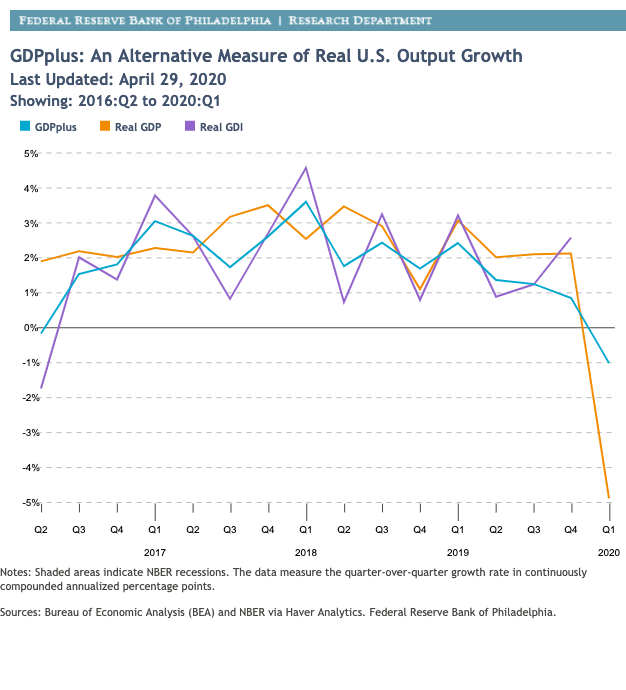
\includegraphics[scale=.5]{GDPplus-20}
\caption{}
\label{gdp-plus}
\end{figure}
\end{proof}
\end{enumerate}
 











\end{document}

